\documentclass[tikz,border=10pt]{standalone}

\usepackage{amsfonts, amsmath, mathrsfs, amssymb, mathdots}

\usetikzlibrary{positioning, backgrounds, shapes.geometric,}


\begin{document}
	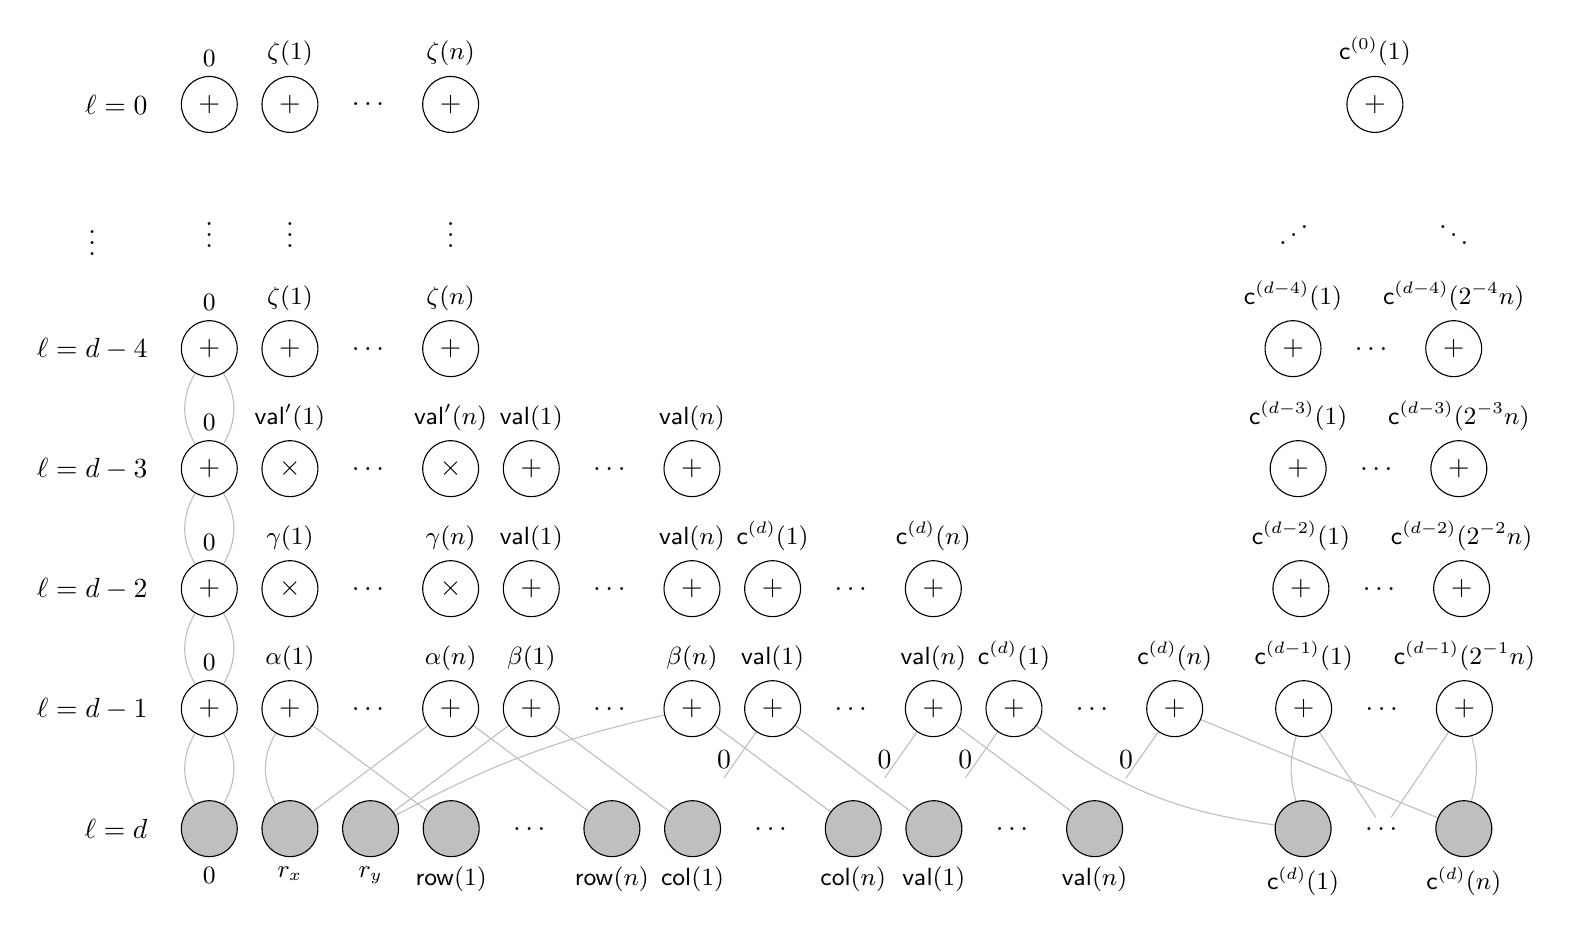
\begin{tikzpicture}[node distance=.8cm and 0.3cm]
		
		\tikzstyle{circleNodeInput} = [circle, draw, fill=lightgray, minimum size=7.1mm,  label={[font=\small]below:#1}]
		
		\tikzstyle{circleNode} = [circle, draw, minimum size=7.1mm, label={[font=\small]above:#1}]
		
		
		
		% % Layer d-4
		
		% \node [circleNode=0, below=of l0zero] (d_4_zero) {+};
		% \node [left=of d_4_zero] (d_4) {Layer $d-4$};
		
		
		
		% Layer d
		
		\node [circleNodeInput=$0$] (dzero) {};
		\node [left=of dzero] (d) {$\ell = d$};
		\node [circleNodeInput=$r_x$, right=of dzero] (d_rx) {};
		\node [circleNodeInput=$r_y$, right=of d_rx] (d_ry) {};
		\node [circleNodeInput=$\mathsf{row}(1)$, right=of d_ry] (d_row_1) {};
		\node [right=of d_row_1] (d_row_dots) {\dots};
		\node [circleNodeInput=$\mathsf{row}(n)$, right=of d_row_dots] (d_row_n) {};
		\node [circleNodeInput=$\mathsf{col}(1)$, right=of d_row_n] (d_col_1) {};
		\node [right=of d_col_1] (d_col_dots) {\dots};
		\node [circleNodeInput=$\mathsf{col}(n)$, right=of d_col_dots] (d_col_n) {};
		\node [circleNodeInput=$\mathsf{val}(1)$, right=of d_col_n] (d_val_1) {};
		\node [right=of d_val_1] (d_val_dots) {\dots};
		\node [circleNodeInput=$\mathsf{val}(n)$, right=of d_val_dots] (d_val_n) {};
		\node [right=of d_val_n, minimum width=13.1mm] (d_space) {};
		\node [circleNodeInput=$\mathsf{c}^{(d)}(1)$, right=of d_space] (d_c_1) {};
		\node [right=of d_c_1] (d_c_dots) {\dots};
		\node [circleNodeInput=$\mathsf{c}^{(d)}(n)$, right=of d_c_dots] (d_c_n) {};
		
		
		% Layer d -1
		\node [circleNode=$0$, above=of dzero] (d_1_zero) {+};
		\node [left=of d_1_zero] (d_1) {$\ell = d-1$};
		\node [circleNode=$\alpha(1)$, right=of d_1_zero] (d_1_alpha_1) {+};
		\node [right=of d_1_alpha_1] (d_1_alpha_dots) {\dots};
		\node [circleNode=$\alpha(n)$, right=of d_1_alpha_dots] (d_1_alpha_n) {+};
		\node [circleNode=$\beta(1)$, right=of d_1_alpha_n] (d_1_beta_1) {+};
		\node [right=of d_1_beta_1] (d_1_beta_dots) {\dots};
		\node [circleNode=$\beta(n)$, right=of d_1_beta_dots] (d_1_beta_n) {+};
		\node [circleNode=$\mathsf{val}(1)$, right=of d_1_beta_n] (d_1_val_1) {+};
		\node [right=of d_1_val_1] (d_1_val_dots) {\dots};
		\node [circleNode=$\mathsf{val}(n)$, right=of d_1_val_dots] (d_1_val_n) {+};
		\node [circleNode=$\mathsf{c}^{(d)}(1)$, right=of d_1_val_n] (d_c_1_copy) {+};
		\node [right=of d_c_1_copy] (d_c_dots_copy) {\dots};
		\node [circleNode=$\mathsf{c}^{(d)}(n)$, right=of d_c_dots_copy] (d_c_n_copy) {+};
		\node [right=of d_c_n_copy, minimum size=3mm] (d_1_space) {};
		\node [circleNode=$\mathsf{c}^{(d-1)}(1)$, right=of d_1_space] (d_1_c_1) {+};
		\node [right=of d_1_c_1] (d_1_c_dots) {\dots};
		\node [circleNode=$\mathsf{c}^{(d-1)}(2^{-1}n)$, right=of d_1_c_dots] (d_1_c_n) {+};
		
		\node [below left=1.5mm and 1.5mm of d_1_val_1] (zero_input_d_1_val_1)  {0}; 
		\node [below left=1.5mm and 1.5mm of d_1_val_n] (zero_input_d_1_val_n)  {0}; 
		
		\node [below left=1.5mm and 1.5mm of d_c_1_copy] (zero_input_d_c_1_copy)  {0}; 
		\node [below left=1.5mm and 1.5mm of d_c_n_copy] (zero_input_d_c_n_copy)  {0}; 
		
		
		% Layer d -2
		\node [circleNode=$0$, above=of d_1_zero] (d_2_zero) {+};
		\node [left=of d_2_zero] (d_2) {$\ell = d-2$};
		\node [circleNode=$\gamma(1)$, right=of d_2_zero] (d_2_gamma_1) {$\times$};
		\node [right=of d_2_gamma_1] (d_2_gamma_dots) {\dots};
		\node [circleNode=$\gamma(n)$, right=of d_2_gamma_dots] (d_2_gamma_n) {$\times$};
		\node [circleNode=$\mathsf{val}(1)$, right=of d_2_gamma_n] (d_2_val_1) {+};
		\node [right=of d_2_val_1] (d_2_val_dots) {\dots};
		\node [circleNode=$\mathsf{val}(n)$, right=of d_2_val_dots] (d_2_val_n) {+};
		\node [circleNode=$\mathsf{c}^{(d)}(1)$, right=of d_2_val_n] (d_2_c_1_copy) {+};
		\node [right=of d_2_c_1_copy] (d_2_c_dots_copy) {\dots};
		\node [circleNode=$\mathsf{c}^{(d)}(n)$, right=of d_2_c_dots_copy] (d_2_c_n_copy) {+};
		\node [right=of d_2_c_n_copy, minimum width=33.3mm] (d_2_space) {};
		\node [circleNode=$\mathsf{c}^{(d-2)}(1)$, right=of d_2_space] (d_2_c_1) {+};
		\node [right=of d_2_c_1] (d_2_c_dots) {\dots};
		\node [circleNode=$\mathsf{c}^{(d-2)}(2^{-2}n)$, right=of d_2_c_dots] (d_2_c_n) {+};
		
		% Layer d -3
		\node [circleNode=$0$, above=of d_2_zero] (d_3_zero) {+};
		\node [left=of d_3_zero] (d_3) {$\ell = d-3$};
		\node [circleNode=$\mathsf{val}^\prime(1)$, right=of d_3_zero] (d_3_val_prime_1) {$\times$};
		\node [right=of d_3_val_prime_1] (d_3_val_prime_dots) {\dots};
		\node [circleNode=$\mathsf{val}^\prime(n)$, right=of d_3_val_prime_dots] (d_3_val_prime_n) {$\times$};
		\node [circleNode=$\mathsf{val}(1)$, right=of d_3_val_prime_n] (d_3_val_1) {+};
		\node [right=of d_3_val_1] (d_3_val_dots) {\dots};
		\node [circleNode=$\mathsf{val}(n)$, right=of d_3_val_dots] (d_3_val_n) {+};
		\node [right=of d_3_val_n, minimum width=63.6mm] (d_3_space) {};
		\node [circleNode=$\mathsf{c}^{(d-3)}(1)$, right=of d_3_space] (d_3_c_1) {+};
		\node [right=of d_3_c_1] (d_3_c_dots) {\dots};
		\node [circleNode=$\mathsf{c}^{(d-3)}(2^{-3}n)$, right=of d_3_c_dots] (d_3_c_n) {+};
		
		% Layer d -4
		\node [circleNode=$0$, above=of d_3_zero] (d_4_zero) {+};
		\node [left=of d_4_zero] (d_4) {$\ell = d-4$};
		\node [circleNode=$\zeta(1)$, right=of d_4_zero] (d_4_zeta_1) {+};
		\node [right=of d_4_zeta_1] (d_4_zeta_dots) {\dots};
		\node [circleNode=$\zeta(n)$, right=of d_4_zeta_dots] (d_4_zeta_n) {+};
		\node [right=of d_4_zeta_n, minimum width=93.6mm] (d_4_space) {};
		\node [circleNode=$\mathsf{c}^{(d-4)}(1)$, right=of d_4_space] (d_4_c_1) {+};
		\node [right=of d_4_c_1] (d_4_c_dots) {\dots};
		\node [circleNode=$\mathsf{c}^{(d-4)}(2^{-4}n)$, right=of d_4_c_dots] (d_4_c_n) {+};
		
		% Layer dots
		\node [above=of d_4_zero] (d_dots_zero) {$\vdots$};
		\node [above=of d_4] (d_dots) {$\vdots$};
		\node [above=of d_4_zeta_1] (d_dots_zeta_1) {$\vdots$};
		% \node [above=of d_4_zeta_dots] (d_dots_zeta_dots) {\vdots};
		\node [above=of d_4_zeta_n] (d_dots_zeta_n) {$\vdots$};
		\node [above=of d_4_c_1] (d_dots_c_1) {$\iddots$};
		\node [above=of d_4_c_n] (d_dots_c_n) {$\ddots$};
		
		% Layer 0
		\node [circleNode=$0$, above=of d_dots_zero] (l_0_zero) {+};
		\node [left=of l_0_zero] (l_0) {$\ell = 0$};
		\node [circleNode=$\zeta(1)$, right=of l_0_zero] (l_0_zeta_1) {+};
		\node [right=of l_0_zeta_1] (l_0_zeta_dots) {\dots};
		\node [circleNode=$\zeta(n)$, right=of l_0_zeta_dots] (l_0_zeta_n) {+};
		\node [right=of l_0_zeta_n, minimum width=104mm] (l_0_space) {};
		\node [circleNode=$\mathsf{c}^{(0)}(1)$, right=of l_0_space] (l_0_c_1) {+};
		
		
		
		% \node [ left=of l0zero] (l0) {Layer 0};
		% \node [circleNode=$\zeta(1)$, right=of l0zero] (l0zita_1) {+};
		% \node [right=of l0zita_1] (l0zita_dots) {\dots};
		% \node [circleNode=$\zeta(n)$, right=of l0zita_dots] (l0zita_n) {+};
		% \node [circleNode=$\mathsf{c}^{(0)}(0)$, right=of l0zita_n] (l0_c_0) {+};
		
		
		
		% ... continue adding nodes ...
		
		% Now, draw the connecting lines if necessary. Since the full pattern of the
		% connections is not clear, I'll just provide a few examples:
		
		\begin{scope}[on background layer]
			\draw[lightgray]  (dzero) to[bend left] (d_1_zero);
			\draw[lightgray]  (dzero) to[bend right] (d_1_zero);
			
			\draw[lightgray]  (d_1_zero) to[bend left] (d_2_zero);
			\draw[lightgray]  (d_1_zero) to[bend right] (d_2_zero);
			
			\draw[lightgray]  (d_2_zero) to[bend left] (d_3_zero);
			\draw[lightgray]  (d_2_zero) to[bend right] (d_3_zero);
			
			\draw[lightgray]  (d_3_zero) to[bend left] (d_4_zero);
			\draw[lightgray]  (d_3_zero) to[bend right] (d_4_zero);
			
			
			\draw[lightgray] (d_rx) to[bend left] (d_1_alpha_1);
			\draw[lightgray] (d_row_1) to (d_1_alpha_1);
			\draw[lightgray] (d_rx) to (d_1_alpha_n);
			\draw[lightgray] (d_row_n) to (d_1_alpha_n);
			
			\draw[lightgray] (d_ry) to (d_1_beta_1);
			\draw[lightgray] (d_col_1) to (d_1_beta_1);
			\draw[lightgray] (d_ry)[bend left=7.5] to (d_1_beta_n);
			\draw[lightgray] (d_col_n) to (d_1_beta_n);
			
			\draw[lightgray]  (d_val_1) to (d_1_val_1);
			\draw[lightgray]  (d_val_n) to (d_1_val_n);
			\draw[lightgray]  (zero_input_d_1_val_1.south) to (d_1_val_1);
			\draw[lightgray]  (zero_input_d_1_val_n.south) to (d_1_val_n);
			
			\draw[lightgray]  (d_c_1)[bend left=15] to (d_c_1_copy);
			\draw[lightgray]  (d_c_n) to (d_c_n_copy);
			\draw[lightgray]  (zero_input_d_c_1_copy.south) to (d_c_1_copy);
			\draw[lightgray]  (zero_input_d_c_n_copy.south) to (d_c_n_copy);
			
			\draw[lightgray]  (d_c_1)[bend left=15] to (d_1_c_1);
			\draw[lightgray]  (d_c_n)[bend right=15] to (d_1_c_n);
			
			\draw[lightgray]  (d_c_dots) to (d_1_c_1);
			\draw[lightgray]  (d_c_dots) to (d_1_c_n);
			
			
			
			
			
			% d_1_c_dots
			
			
			% \node (intermediate) at (1.5, .75) {}; % Intermediate control point
			% \draw[lightgray] (dzero) to[bend left=20] (intermediate) to[bend right=10] (d_1_val_n);
			
			% \draw[lightgray] (dzero) to[bend left=20] (intermediate) to[bend right=15] (d_1_val_1);
			
			
			% \draw[lightgray] (intermediate) to[bend right=10] (d_1_val_n);
			% \draw[lightgray] (intermediate) to[bend right=20] (d_1_val_1);
			
			
			
		\end{scope}
		% \draw (d4zero2) -- (d3c1);
		% ... continue drawing connections ...
		
		% Add other layers with labels below the nodes in a similar manner.
		% ...
		
	\end{tikzpicture}
\end{document}
